\subsection{Demonstration of \cegiw{} (RQ1)}\label{subsec:demonstration}

To address \textbf{RQ1}, we use an example based on a model of a foraging robot swarm~\cite{liu2010}. Robots are located in an arena and do a random walk to find food, which they then carry back to their home. Here they recharge and then repeat their foraging task. We model a single robot with a state machine, depicted abstractly in \cref{fig:foraging-fsm}.
%
\begin{figure}[t]
\centering
\begin{tikzpicture}[node distance=1.5cm and 3.5cm, on grid, auto]
\node[state] (deposit) {\texttt{deposit}};
\node[state, above=of deposit] (movetohome) {\texttt{moveToHome}};
\node[state, right=of movetohome] (grabfood) {\texttt{grabFood}};
\node[state, right=of grabfood] (movetofood) {\texttt{moveToFood}};
\node[state, right=of deposit] (homing) {\texttt{homing}};
\node[state, right=of homing] (scanarena) {\texttt{scanArena}};
\node[state, below=of deposit] (resting) {\texttt{resting}};
\node[left=5em of resting] (inv1) {};
\node[state, right=of resting] (leavinghome) {\texttt{leavingHome}};
\node[state, right=of leavinghome] (randomwalk) {\texttt{randomWalk}};

\path[->]
    (inv1) edge (resting)
    (resting) edge (leavinghome)
    (leavinghome) edge (randomwalk)
    (randomwalk) edge (homing)
    (homing) edge (resting)
    (randomwalk) edge[bend right=75](movetofood)
    (movetofood) edge (homing)
    (movetofood) edge[bend right=20] (scanarena)
    (scanarena) edge[bend right=20] (movetofood)
    (scanarena) edge (randomwalk)
    (movetofood) edge (grabfood)
    (grabfood) edge (movetohome)
    (movetohome) edge (deposit)
    (deposit) edge (resting);
\end{tikzpicture}
\caption{Abstract state transition system for the robot's foraging behaviour. The robot begins in a resting state, then searches for, collects, and deposits food.}
\label{fig:foraging-fsm}
\end{figure}
%
% \marienote{this caption could be a bit more descriptive: The robot begins in a resting state, then proceeds to walk around the arena, scanning, searching for, collecting and depositing food items...}
%
In the concrete transition system $\mathcal{M}$ the robot can remain in a given state for a configurable amount of time before it is forced to move to a next state. The transition system is specified concretely using \SMV{}, the language of the \nuXmv{} model checker~\cite{cavada2014}. We would like to prove that, after leaving the \texttt{resting} state, the robot will return to \texttt{resting} in at most 3 time units, represented by
%
\begin{equation}\label{eqn:max-return-to-resting-mtl}
\mathcal{M}\vDash\Box(\texttt{resting} \rightarrow \eventually{[1,3]}\texttt{resting})
\end{equation}
% \centereqn{\mathcal{M}\vDash\Box(\texttt{resting} \rightarrow \eventually{[1,3]}\texttt{resting})\label{eqn:max-return-to-resting-mtl}}
%
and translated from \MTL{} to \LTL{} as
%
\begin{equation}\label{eqn:max-return-to-resting-ltl}
\mathcal{M}\vDash\Box(\texttt{resting} \rightarrow X(\texttt{resting} \lor X(\texttt{resting} \lor X(\texttt{resting})))).
\end{equation}
% \centereqn{\mathcal{M}\vDash\Box(\texttt{resting} \rightarrow X(\texttt{resting} \lor X(\texttt{resting} \lor X(\texttt{resting})))).\label{eqn:max-return-to-resting-ltl}}
%
If this does not hold in the transition system, we would like to weaken the interval to produce a new, weaker property that does hold. Using \cegiw{}, we find in the first iteration that no suitable weakening of the interval exists based on the counterexample in \cref{fig:min-to-resting-cex}, which shows an infinite loop between the \texttt{scanArena} and \texttt{moveToFood} states. This suggests a mistake in the modelling of the system, as in the real world the robot's battery would run out of charge.
%
\begin{figure}[t]
\centering
% \begin{verbatim}
%                0 1 2 3 4 5
%   resting     │+│ │ │ │ │ │
%   leavingHome │ │+│ │ │ │ │
%   randomWalk  │ │ │+│ │ │ │
%   moveToFood  │ │ │ │+│ │+│
%   scanArena   │ │ │ │ │+│ │
%   =Lasso=              └─┘
% \end{verbatim}
\begin{tikzpicture}[auto,node distance=4mm]
\node[cex] (1) {\scriptsize\texttt{resting}};
\node[left=of 1] (inv1) {};
\node[cex, right=of 1] (2) {\scriptsize\texttt{leavingHome}};
\node[cex, right=of 2] (3) {\scriptsize\texttt{randomWalk}};
\node[cex, right=of 3] (4) {\scriptsize\texttt{moveToFood}};
\node[cex, right=of 4] (5) {\scriptsize\texttt{scanArena}};
\node[cex, right=of 5] (6) {\scriptsize\texttt{moveToFood}};
\node[right=of 6] (inv2) {};

\path[->]
    (inv1) edge (1)
    (1) edge (2)
    (2) edge (3)
    (3) edge (4)
    (4) edge (5)
    (5) edge (6)
    (6) edge[bend right=325] (4);
\end{tikzpicture}
\caption{Infinite lasso counterexample trace for the property in \cref{eqn:max-return-to-resting-mtl}.}
\label{fig:min-to-resting-cex}
\end{figure}
%
We amend the design by including in the requirements the notion of a battery that decreases as transitions are taken. While we are in \texttt{randomWalk}, \texttt{scanArena}, or \texttt{moveToFood} --- in other words, searching for food --- we monitor the battery level, and if it decreases below a certain threshold we abort and return home to recharge. The modified state transition system is depicted in \cref{fig:foraging-fsm-modified}.
%
\begin{figure}[t]
\centering
\begin{tikzpicture}[node distance=1.5cm and 3.5cm, on grid, auto]
\draw[thick,dashed] ($(movetofood.north west)+(-0.3,0.3)$) rectangle ($(randomwalk.south east)+(0.3,-0.3)$) node [midway, above=2.25] {\texttt{battery monitor}};
\draw[->,thick,dashed] ($($($(movetofood.north west)+(-0.3,0)$)!0.5!($(randomwalk.south west)+(-0.3,0)$)$)$) -- (homing) node [midway, below] {\texttt{abort}};
\node[state] (deposit) {\texttt{deposit}};
\node[state, above=of deposit] (movetohome) {\texttt{moveToHome}};
\node[state, right=of movetohome] (grabfood) {\texttt{grabFood}};
\node[state, right=of grabfood] (movetofood) {\texttt{moveToFood}};
\node[state, right=of deposit] (homing) {\texttt{homing}};
\node[state, right=of homing] (scanarena) {\texttt{scanArena}};
\node[state, below=of deposit] (resting) {\texttt{resting}};
\node[left=5em of resting] (inv1) {};
\node[state, right=of resting] (leavinghome) {\texttt{leavingHome}};
\node[state, right=of leavinghome] (randomwalk) {\texttt{randomWalk}};

\path[->]
    (inv1) edge (resting)
    (resting) edge (leavinghome)
    (leavinghome) edge (randomwalk)
    (randomwalk) edge (homing)
    (homing) edge (resting)
    (randomwalk) edge[bend right=75](movetofood)
    (movetofood) edge (homing)
    (movetofood) edge[bend right=20] (scanarena)
    (scanarena) edge[bend right=20] (movetofood)
    (scanarena) edge (randomwalk)
    (movetofood) edge (grabfood)
    (grabfood) edge (movetohome)
    (movetohome) edge (deposit)
    (deposit) edge (resting);
\end{tikzpicture}
\caption{Abstract state transition system for the robot's modified foraging behaviour. The battery monitor is represented by the dashed section on the right.}
\label{fig:foraging-fsm-modified}
\end{figure}
%
\begin{figure}[t]
\centering
\begin{subfigure}[t]{0.5\textwidth}
    \centering
    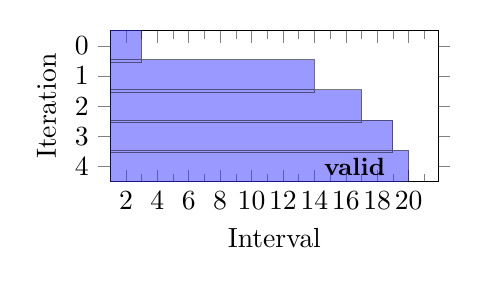
\begin{tikzpicture}
    \begin{axis}[
        xbar,
        xmin=1,
        width=5.75cm,
        height=3.5cm,
        xlabel={Interval},
        ylabel={Iteration},
        ytick=data,
        xtick distance=2,
        minor x tick num=1,
        x tick label as interval=false,
        y dir=reverse,
        ymin=-0.5,
        ymax=4.5,
        bar width=1.18em,
    ]
    \addplot+[black,fill=blue!80!white,opacity=0.5] coordinates {(20,4) (19,3) (17,2) (14,1) (3,0)};
    \node[
        anchor=west,
        font=\small,
    ] at (axis cs:14,4) {\textbf{valid}};
    \end{axis}
    \end{tikzpicture}
    \caption{Interval extension for \cref{eqn:max-return-to-resting-mtl}.}
    \label{fig:iterative-interval-extension}
\end{subfigure}%
\begin{subfigure}[t]{0.5\textwidth}
    \centering
    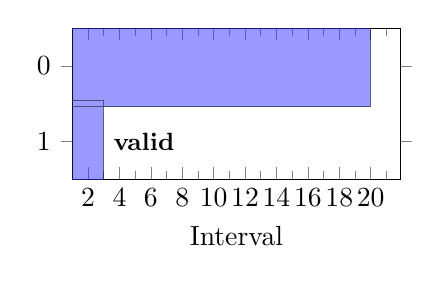
\begin{tikzpicture}
    \begin{axis}[
        xbar=1em,
        xmin=1,
        width=5.75cm,
        height=3.5cm,
        xlabel={Interval},
        ytick=data,
        xtick distance=2,
        minor x tick num=1,
        x tick label as interval=false,
        y dir=reverse,
        ymin=-0.5,
        ymax=1.5,
        bar width=2.95em,
    ]
    \addplot+[black,fill=blue!80!white,opacity=0.5] coordinates {(20,0) (3,1)};
    \node[
        anchor=west,
        font=\small,
    ] at (axis cs:3,1) {\textbf{valid}};
    \end{axis}
    \end{tikzpicture}
    \caption{Interval contraction for \cref{eqn:min-return-to-resting}.}
    \label{fig:iterative-interval-contraction}
\end{subfigure}
\caption{Iterative interval weakening to generate optimal, valid intervals.}
\end{figure}
%
We check our desired property (\cref{eqn:max-return-to-resting-mtl}) against our amended model, and can see in \cref{fig:iterative-interval-extension} that in four iterations of \cegiw{} we extended the interval, and ended with the optimal interval which was then verified to hold in the system. So, the optimal property that holds in our amended system is
\begin{equation}\label{eqn:max-return-to-resting-corrected}
    \mathcal{M}\vDash\Box(\texttt{resting} \rightarrow \eventually{[1,20]}\texttt{resting}).
\end{equation}
%
Another property we are interested in is not the maximum time that the robot can spend away from home, but the \emph{minimum}. We wish the robot to spend at least 20 time units away from home, formalised as
%
\begin{equation}\label{eqn:min-return-to-resting}
\mathcal{M}\vDash\Box((\texttt{resting}\land\eventually{[1,1]}\neg\texttt{resting}) \rightarrow \generally{[1,20]}\neg\texttt{resting}).
\end{equation}
%
Again, we check this against our modified model and can see in \cref{fig:iterative-interval-contraction} that it took only one iteration to contract the interval, reaching the optimal interval which was then verified to hold in the system as
%
\begin{equation}\label{eqn:min-return-to-resting-corrected}
\mathcal{M}\vDash\Box((\texttt{resting}\land\eventually{[1,1]}\neg\texttt{resting}) \rightarrow \generally{[1,3]}\neg\texttt{resting}).
\end{equation}
%
By using \cegiw{}, we first identified that the original specification had a design flaw that allowed unwanted infinite loops. After modifying the specification, we then deduced both the maximum time that the robot can stay away from home, as well as the minimum time.
